\subsection{Algorithmus}\label{subsec:algorithmus}

\paragraph{AVL-Bedingung}
Ein AVL-Baum ist ein Binärbaum, der die zusätzliche Eigenschaft besitzt, dass
die Balance, die als die Differenz der Höhe $h$ der beiden
Teilbäume definiert ist (siehe Formel~\ref{eq:balance}), bei jedem Knoten mindestens 1 und
maximal 1 beträgt.
Diese Eigenschaft wird AVL-Bedingung genannt.
Dabei ist die Höhe analog zum regulären Binärbaum definiert (siehe Formel~\ref{eq:height}).

\begin{equation}
    bal(k) = h(T_r) - h(T_l)\label{eq:balance} \in \{-1,0,1\}
\end{equation}
\begin{equation}
    h(k) = max(h(T_l), h(T_r))\label{eq:height}
\end{equation}
Durch diese Bedingung wird sichergestellt, dass der Baum zu jedem Zeitpunkt
balanciert ist und somit das in der Einleitung beschriebene Problem der
schlechten Laufzeit des Binärbaumes durch Entartung nicht auftreten kann.

\paragraph{Rebalancierung}\label{par:rebalancing}
Nach dem Einfügen und Löschen von Elementen kann es jeweils vorkommen, dass die
Balance eines Konten -2 oder 2 beträgt.
Somit muss der AVL-Baum nach diesen Operationen die AVL-Bedingung überprüfen,
und eventuell eine Rebalancierung vornehmen.
Dabei wird zwischen insgesamt vier Fällen unterschieden, die durch die Folge
der Balancewerte definiert sind (siehe auch Abbildung~\ref{fig:AVL-Cases}):
\begin{enumerate}
    \item Left Left: -2/-1 oder -2/0 → Rechtsrotation\label{enm:rebal1}
    \item Right Right: +2/+1 oder +2/0 → Linksrotation \label{enm:rebal2}
    \item Left Right: -2/+1 → Doppelte Rechtsrotation \label{enm:rebal3}
    \item Right Left: +2/-1 → Doppelte Linksrotation \label{enm:rebal4}
\end{enumerate}
Die ersten beiden und letzten beiden Fälle sind dabei jeweils symmetrisch zueinander.

\paragraph*{Rotation}

Bei einer Rotation wird immer ein Knoten als Wurzelknoten betrachtet.
Alle Knoten, die über dem Wurzelknoten stehen, sind für die Rotation nicht von
Relevanz.
%Im Left Left bzw. Right Right Case ist dies der Knoten,
%bei dem die AVL-Bedingung verletzt wird.
Der Wurzelknoten wird mit dem Kindknoten rotiert, auf dessen Seite die
Unbalance vorliegt, im Folgenden wird dieses Kind Rotationsknoten genannt:
\begin{itemize}
    \item Linksrotation: Bei positiver Balance mit dem rechten Kindknoten
    \item Rechtsrotation: Bei negativer Balance mit dem linken Kindknoten
\end{itemize}
Betrachte Abbildung~\ref{fig:AVL-Cases}~(Left~Left~Case).
Zum Rotieren der beiden Knoten nach rechts werden folgende Operationen ausgeführt:
\begin{enumerate}
    \item Der Wurzelknoten (5) wird als rechtes Kind vom Rotationsknoten (4)
    gesetzt\label{enm:reblStep1}
    \item Der eben ersetzte Knoten (C) (rechtes Kind vom Rotationsknoten) wird als linkes Kind
    des ursprünglichen Wurzelknotens (5) gesetzt\label{enm:reblStep2}
    \item Der Rotationsknoten (4) wird als neue Wurzel gesetzt\label{enm:reblStep3}
\end{enumerate}
Dabei muss die Höhe des Rotations- und Wurzelknotens angepasst werden.
Dies lässt sich am leichtesten durch eine erneute Berechnung mit Formel~\ref{eq:height} erzielen.

%TODO Formel machen
Die Operation~\ref{enm:reblStep1} ist erlaubt, da (5) größer als (4) sein muss, somit als rechtes
Kind von (4) gesetzt werden kann.
Die Operation~\ref{enm:reblStep2} ist erlaubt, da (C) größer als (4) aber kleiner als (5) sein
muss, somit als rechtes Kind von (4) gesetzt werden kann.
An Abbildung~\ref{fig:AVL-Cases}~(Balanced) wird deutlich, dass durch die
Rechtsrotation beim Left Left Case die AVL-Bedingung wieder erfüllt ist.

Eine Linksrotation erfolgt symmetrisch.

\paragraph{Doppelrotation}

Bei den Fällen Left Left und Right Right konnte der Baum mit lediglich
einer Rotation balanciert werden.
Dies reicht bei den anderen Fällen nicht aus, wie wird aus Abbildung~\ref{fig:AVL-wrong-rotate}
ersichtlich wird.

Es müssen insgesamt zwei Rotationen durchgeführt werden:
Mit der ersten Rotation wird der Left Left bzw. Right Right Case
herbeigeführt, die zweite Rotation befriedigt anschließen die AVL-Bedingung.
Betrachte Abbildung~\ref{fig:AVL-Cases} (Left Right Case).
Im Left Right Case wird zunächst eine Linksrotation zwischen dem linken
Kindknoten des Wurzelelementes und des rechten Nachfolgers ausgeführt.
Diese Rotation wird symmetrisch zur oben beschriebenen Rechtsrotation ausgeführt.
Anschließend liegt der Left Left Case vor, eine einfache Rechtsrotation
befriedigt nun die AVL-Bedingung.


\begin{figure}[hbt]
    \centering
    %https://fr.m.wikipedia.org/wiki/Fichier:AVL_Tree_Rebalancing.svg
    %https://github.com/LambdaSchool/Data-Structures
    %https://commons.wikimedia.org/wiki/File:AVL_Tree_Rebalancing_he.svg
    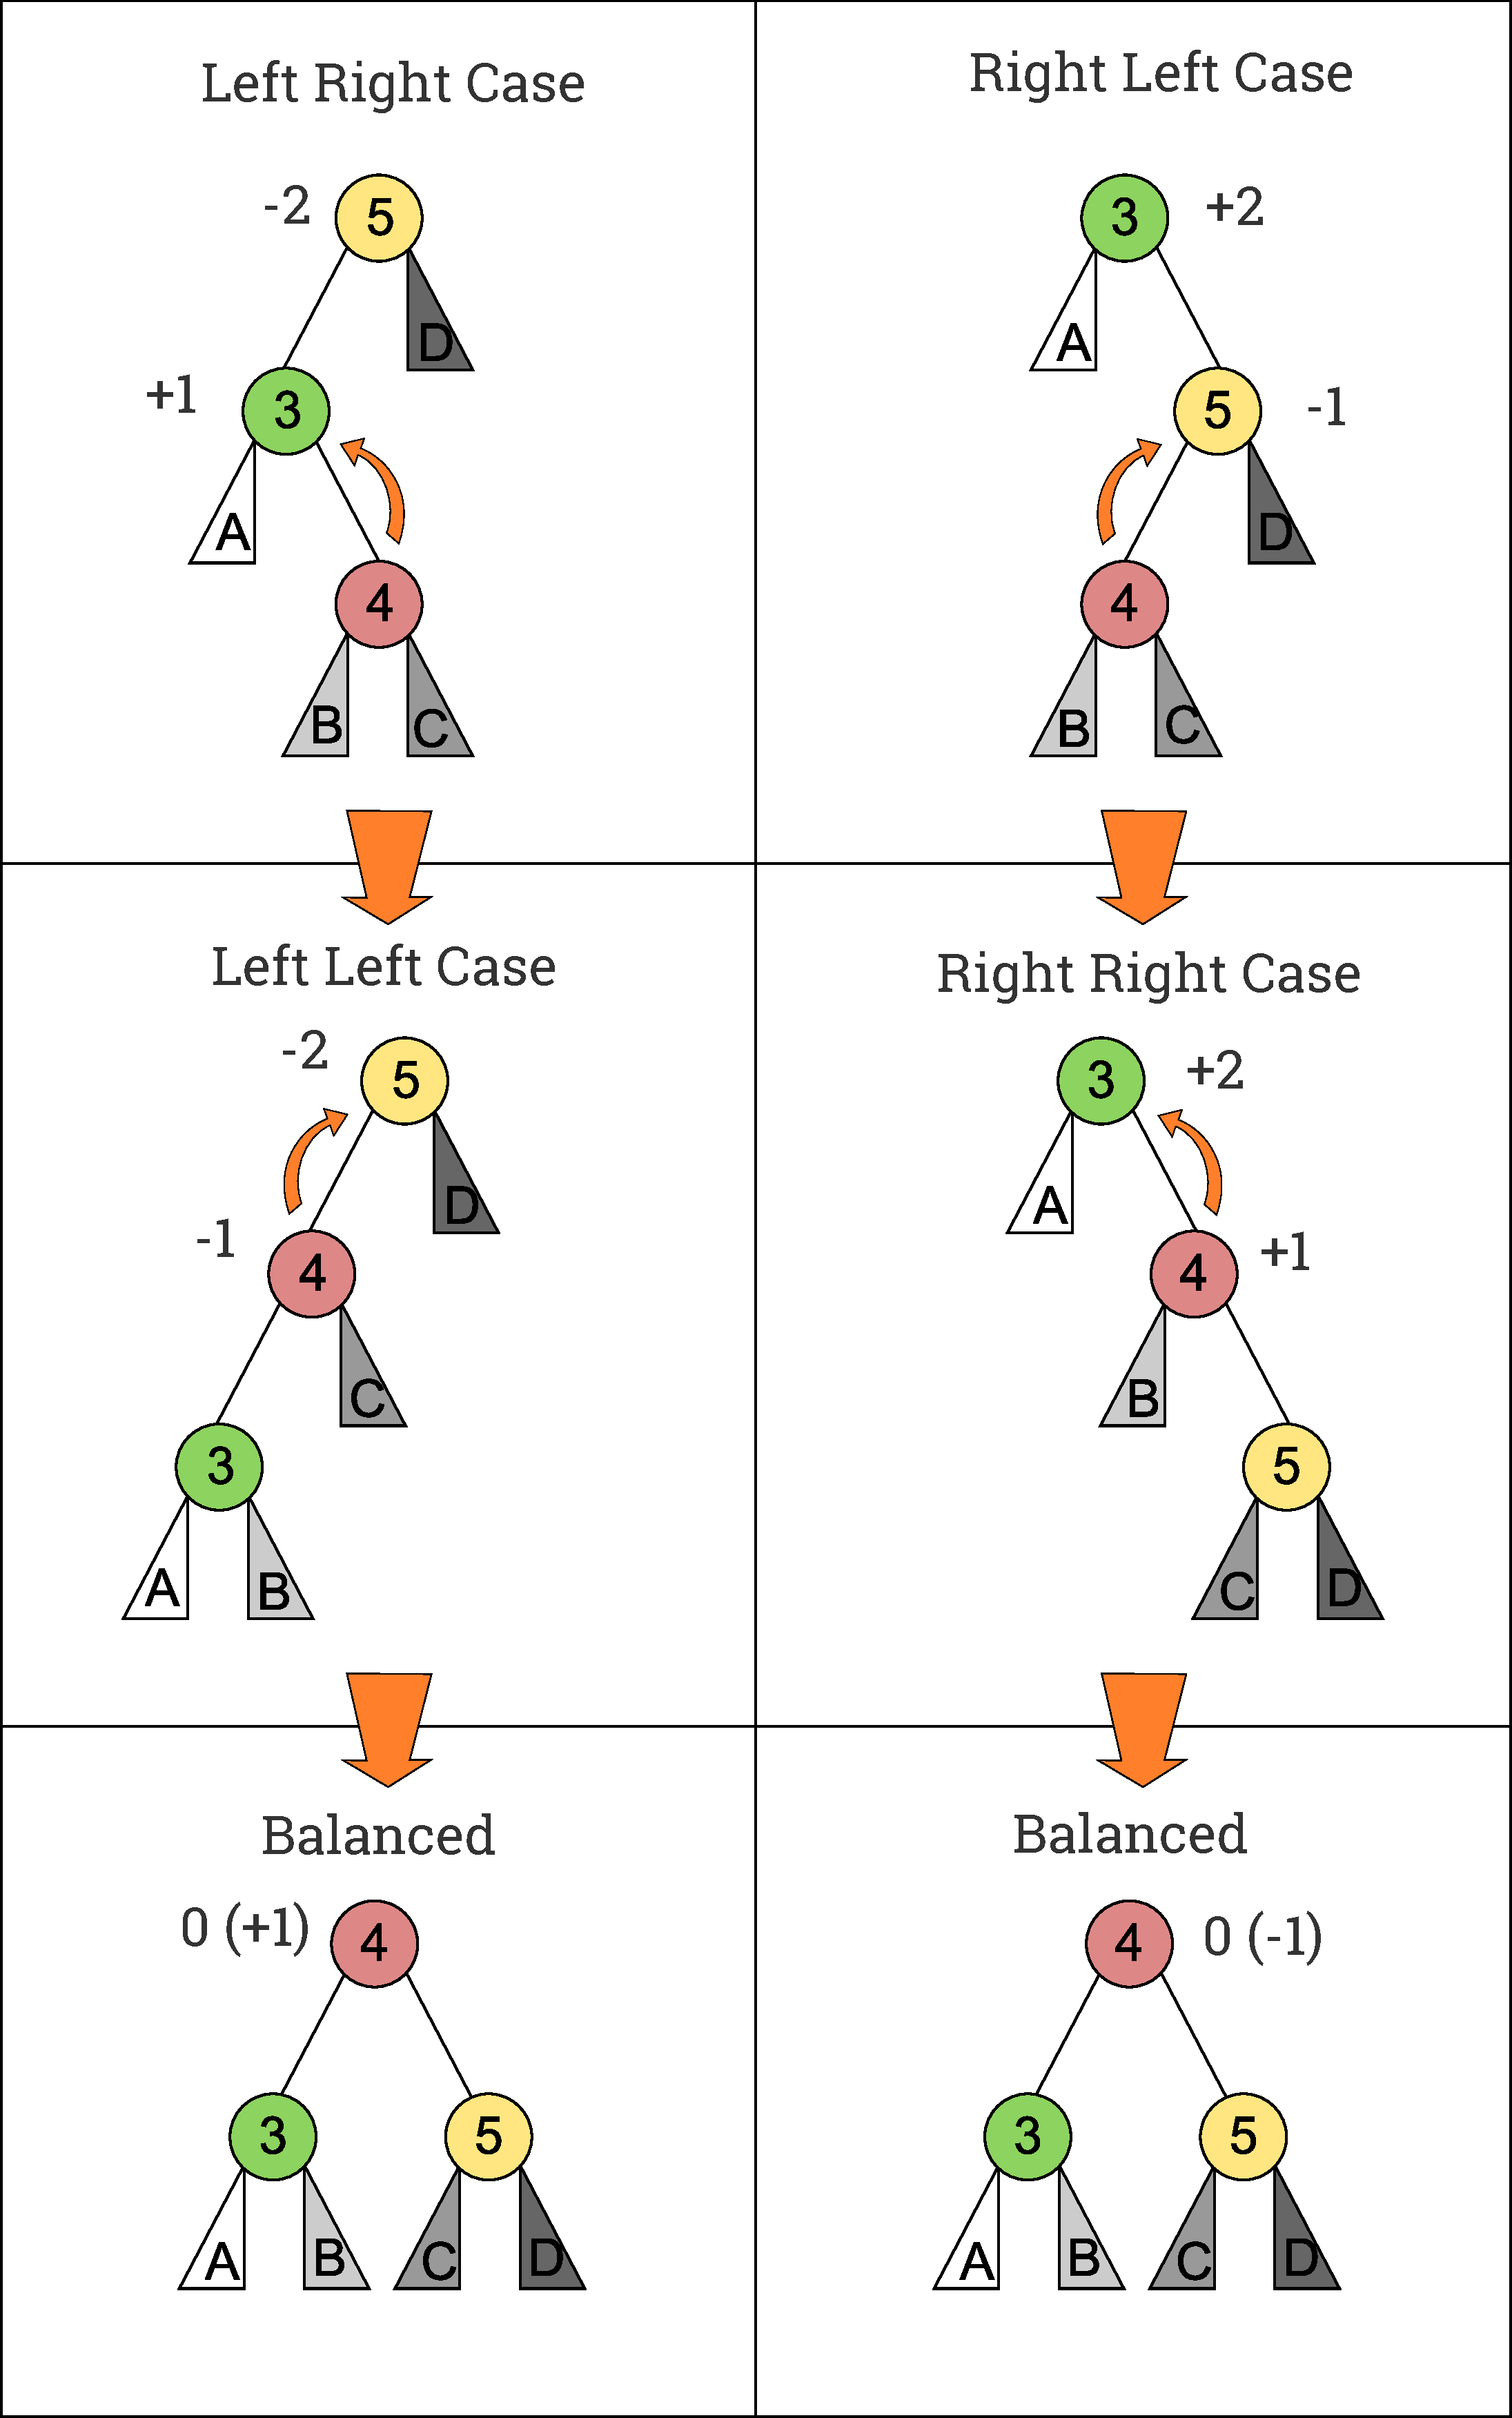
\includegraphics[width= 0.5\textwidth]{img/AVL_Tree_Rebalancing}
    \caption{Rebalancierung}
    \label{fig:AVL-Cases}
\end{figure}
\begin{figure}[hbt]
    \centering
    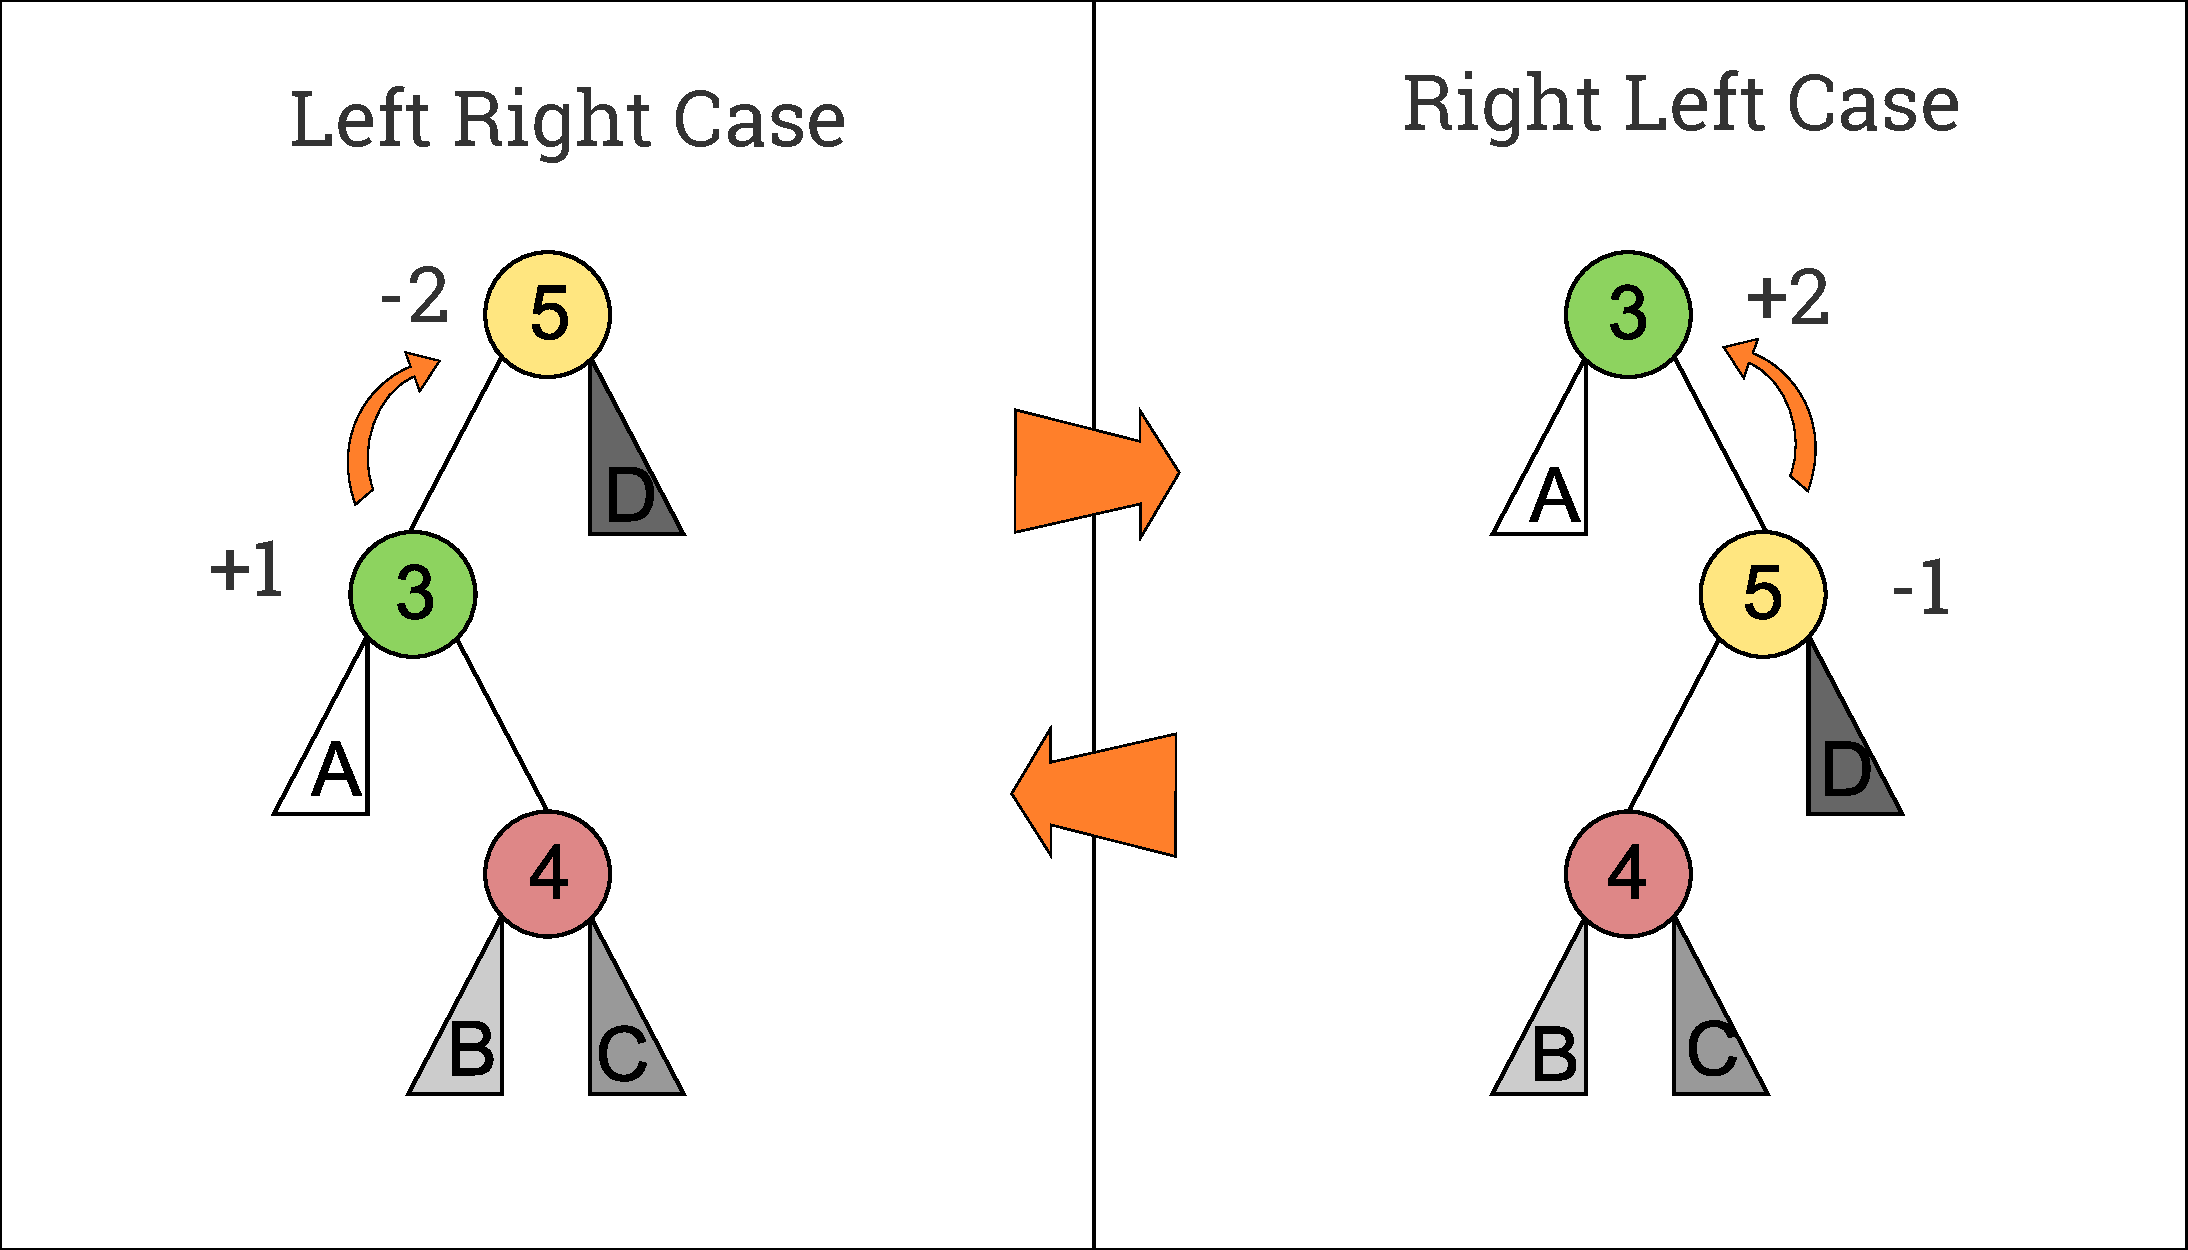
\includegraphics[width= 0.5\textwidth]{img/AVL_Tree_Rebalancing_wrong.pdf}
    \caption{Falsche Rotation}
    \label{fig:AVL-wrong-rotate}
\end{figure}

\subsection{Entwurf}\label{subsec:entwurf2}

\paragraph{InitBT, IsEmptyBT, EqualBT, FindBT}
Die Implementation dieser Methoden kann aus der ersten Praktikumsaufgabe übernommen werden.

\paragraph{IsBT}
Die Methode aus der ersten Praktikumsaufgabe wird um die Überprüfung der
AVL-Bedingung erweitert.
Dabei wird bei jedem Knoten zusätzlich überprüft, ob die Balance (siehe Formel~\ref{eq:balance})
-1, 0 oder +1 beträgt.
Der Ausdruck wird mit den bisherigen Ausdrücken und-verknüpft.

\paragraph{InsertBT, DeleteBT}
Das Einfügen und Löschen wird wie bei einem Binärbaum realisiert.
Die einzige Änderung, die vorgenommen werden muss, ist das Prüfen der
AVL-Bedingung und eventuelles Rotieren, bottom-up nach dem Einfügen bzw. Löschen.
Diese wird mithilfe der \verb|Rebalance|-Methode vorgenommen, die in
Abschnitt~\nameref{par:MethodRebalance} weiter ausgeführt wird.
Beim Löschen muss darauf geachtet werden, dass der Pfad vom tatsächlich entfernten Knoten, also
dem Substitution-Knoten, überprüft wird.
In Abbildung~\ref{fig:AVL-insert} und~\ref{fig:AVL-delete} sind die notwendigen Änderungen jeweils
grün markiert.

\begin{figure}[p]
    \centering
    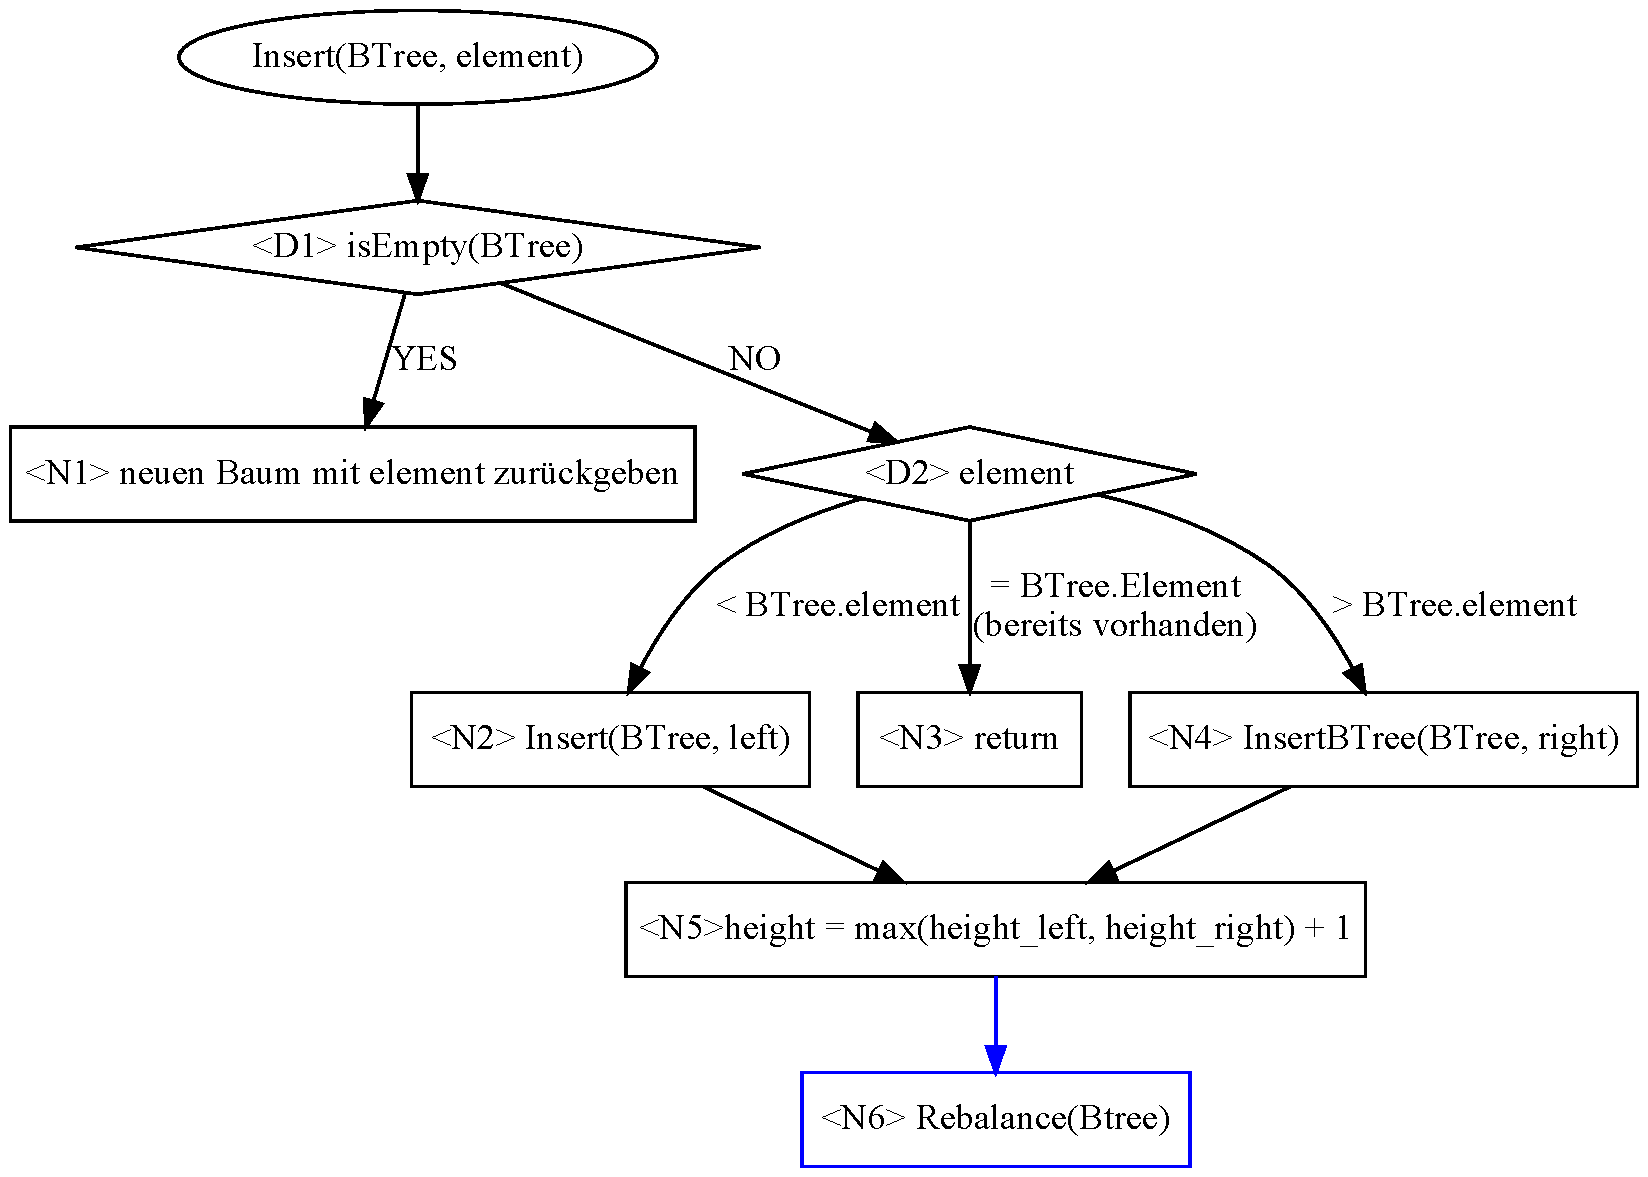
\includegraphics[width= 1.0\textwidth]{img/insert}
    \caption{InsertBT}
    \label{fig:AVL-insert}
\end{figure}
\begin{figure}[p]
    \centering
    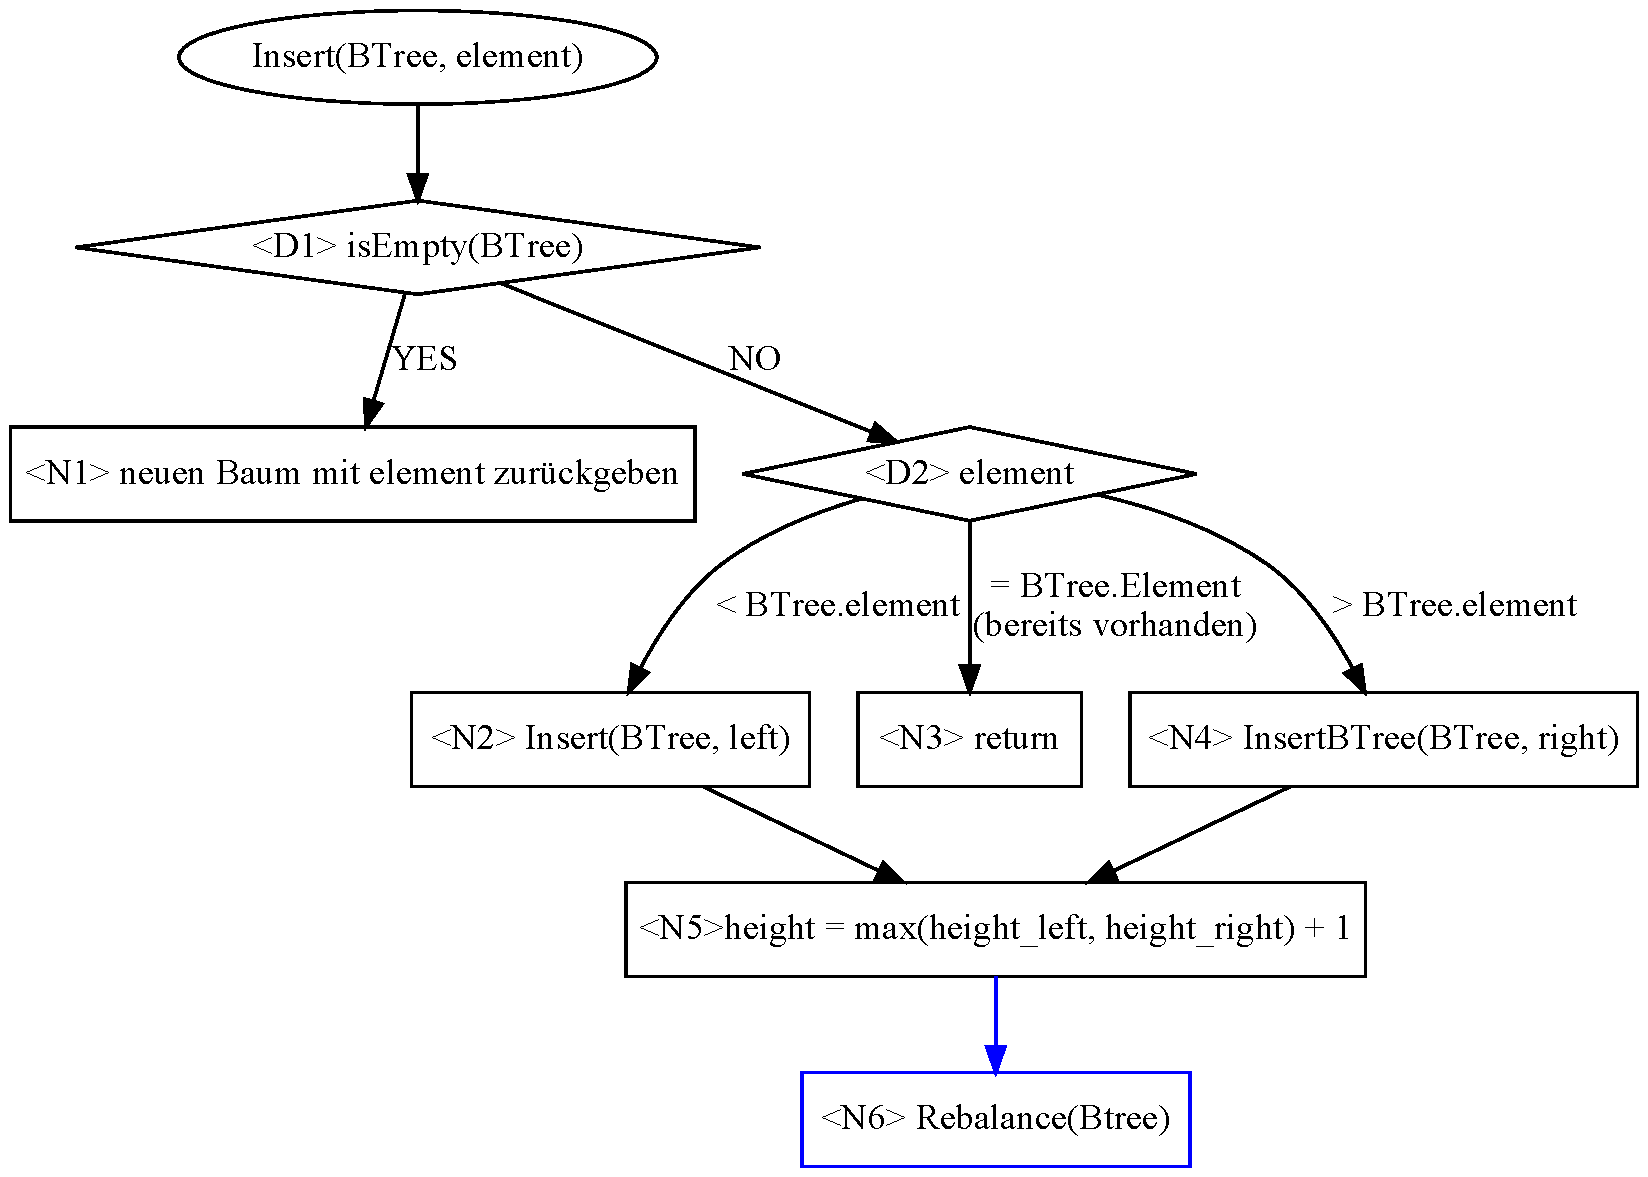
\includegraphics[width= 1.0\textwidth]{img/insert}
    \caption{DeleteBT}
    \label{fig:AVL-delete}
\end{figure}

\paragraph{PrintBT}
Diese Funktion speichert eine Datei im GraphViz Format, welche den Baum darstellt.
Dafür muss am Anfang einmal der Header (\verb|digraph G{|), dann der Inhalt, am Ende eine
schließende Klammer ausgegeben.
Um den Inhalt auszugeben werden für jeden Knoten bis zu zwei Zeilen ausgegeben:
\begin{enumerate}
    \item \verb|<Vater> -> <Linkes Kind> [label = <Hoehe Linkes Kind>];|
    \item \verb|<Vater> -> <Rechtes Kind> [label = <Hoehe Rechtes Kind>];|
\end{enumerate}
Dabei entspricht \verb|Vater, Linkes Kind, Rechtes Kind| dem Wert des jeweiligen Knotens.
Falls ein Kindknoten leer sein sollte, wird dafür keine Zeile ausgegeben.

\paragraph{Rebalance(BTree)}\label{par:MethodRebalance}
Die \verb|Rebalance|-Methode bekommt einen Knoten übergeben, überprüft die Balance und balanciert
den Knoten durch Rotieren, falls diese nicht gegeben ist.
Dafür wird zunächst die Balance des übergebenen Knotens überprüft.
Falls diese -1, 0, +1 beträgt, wird der Knoten nicht verändert.
Andernfalls wird überprüft, welcher der in Abschnitt \nameref{par:rebalancing} aufgeführten Fälle
vorliegt und die nötigen Rotationen mithilfe der \nameref{par:MethodRotate}-Methode ausgeführt.
Falls

\paragraph{Rotate(BTree, Direction)}\label{par:MethodRotate}

\subsection{Aufgaben}

\paragraph{Aufgabe 1.5: Löschen von 88 Prozent der Zahlen}
Es wird ein Baum aus 100 Zufallszahlen erstellt, anschließen werden zufällig 88 davon wieder
gelöscht.
In Abbildung~\ref{fig:88before} ist der Baum vor dem Löschen zu sehen.
In Abbildung~\ref{fig:88after} ist der Baum nach dem Löschen zu sehen.

\begin{figure}[hbtp]\label{fig:88before}
    \centerline{\includegraphics[width = 1.2\textwidth,center]{img/1_6_before.pdf}}
        \caption{Vor dem Löschen}
\end{figure}
\begin{figure}[hbtp]\label{fig:88after}
\centering
        \includegraphics[width = 0.25\textwidth]{img/1_6_after.pdf}
        \caption{Nach dem Löschen}
\end{figure}
